%%% CS6002 Project Report (AAMAS-style)
%%% No-Regret Learning in Stackelberg Security Games with an Unknown,
%%% Bounded Set of Attacker Types.
%%%
%%% Structure follows report_instructions.txt and visual format follows the
%%% AAMAS sigconf look of p597.pdf (two columns, tight margins, amsthm, natbib).

\documentclass[letterpaper,9pt,twocolumn]{extarticle}

\usepackage[top=0.85in,bottom=1in,left=0.7in,right=0.7in,columnsep=0.3in]{geometry}
\usepackage[utf8]{inputenc}
\usepackage[T1]{fontenc}
\usepackage{lmodern}
\usepackage{microtype}

\usepackage{amsmath,amssymb,amsthm}
\usepackage{mathtools}
\usepackage{bm}
\usepackage{graphicx}
\usepackage{booktabs}
\usepackage{algorithm}
\usepackage{algpseudocode}
\usepackage{enumitem}
\usepackage{xcolor}
\usepackage[hidelinks,breaklinks=true]{hyperref}
\usepackage[capitalise,noabbrev]{cleveref}
\usepackage[square,sort&compress,numbers]{natbib}
\bibliographystyle{abbrvnat}

% ---- Balcan et al. notation (Balcan, Blum, Haghtalab, Procaccia 2015) ----
\newcommand{\pvec}{\mathbf{p}}
\newcommand{\svec}{\mathbf{s}}
\newcommand{\avec}{\mathbf{a}}
\newcommand{\cP}{\mathcal{P}}
\newcommand{\cE}{\mathcal{E}}
\newcommand{\cD}{\mathcal{D}}
\newcommand{\cC}{\mathcal{C}}
\newcommand{\cM}{\mathcal{M}}
\newcommand{\EE}{\mathbb{E}}
\newcommand{\NN}{\mathbb{N}}
\newcommand{\RR}{\mathbb{R}}
\newcommand{\Kmax}{K_{\max}}
\newcommand{\Nmax}{N_{\max}}
\newcommand{\argmax}{\operatorname*{arg\,max}}
\newcommand{\argmin}{\operatorname*{arg\,min}}
\newcommand{\Regret}{\mathrm{Regret}}

% ---- Theorem environments ----
\theoremstyle{plain}
\newtheorem{theorem}{Theorem}
\newtheorem{lemma}[theorem]{Lemma}
\newtheorem{proposition}[theorem]{Proposition}
\newtheorem{corollary}[theorem]{Corollary}
\theoremstyle{definition}
\newtheorem{definition}[theorem]{Definition}
\newtheorem{problem}[theorem]{Problem}
\theoremstyle{remark}
\newtheorem{remark}[theorem]{Remark}

% ---- Header ----
\usepackage{fancyhdr}
\pagestyle{fancy}
\fancyhf{}
\renewcommand{\headrulewidth}{0pt}
\fancyfoot[C]{\thepage}

% ---- Title block ----
\title{\vspace{-2em}\textbf{\LARGE No-Regret Learning in Stackelberg Security Games\\
with an Unknown, Bounded Set of Attacker Types}}
\author{\normalsize
\begin{tabular}{ccc}
Aditi Singh & Ishita & Sabil Ahmad
\end{tabular}\\[0.2em]
\footnotesize\textit{Indian Institute of Technology Bombay}\\[0.1em]
\footnotesize CS\,6002 Project Report,  Spring 2026}
\date{\vspace{-1em}}

\begin{document}
\twocolumn[
  \begin{@twocolumnfalse}
  \maketitle
  % \begin{abstract}
% Stackelberg Security Games (SSGs) model the strategic allocation of limited
% defender resources against attackers whose preferences are often uncertain.
% \citet{balcan2015} designed no-regret online learning algorithms for the
% \emph{repeated} variant of SSGs against an adversarial sequence of attackers
% drawn from a finite, \emph{known} set $K$, and proved a matching linear-regret
% lower bound when $K$ is unbounded. A natural real-world middle ground is
% left open: the defender does not know $K$ a priori, but has a bound $\Kmax$
% on its size. We study this setting in the full-information feedback model.
% We propose \textsc{Grow-Catalogue}, an algorithm that incrementally learns
% new attacker types as they arrive, re-partitions the coverage polytope, and
% runs an anytime multiplicative-weights sub-routine on the resulting
% extreme-point set. Our central technical contribution is a full proof that
% \textsc{Grow-Catalogue} achieves expected regret
% \[
% O\!\left(\sqrt{T\cdot\Kmax\cdot(n^2+\Kmax\log n)}\right)
% \]
% against any oblivious adversarial sequence of length $T$. The rate matches
% that of \citet{balcan2015} with $k$ replaced by $\Kmax$ and is sublinear
% whenever $\Kmax\cdot(n^2+\Kmax\log n)=o(T)$. Experiments on synthetic SSG
% instances confirm the predicted $\sqrt{T}$ scaling, and the empirical regret
% stays comfortably below the analytic $C\sqrt{T}$ envelope. Code is available
% at \textcolor{blue}{\href{https://github.com/CS6002-SSG/grow-catalogue}{github.com/CS6002-SSG/grow-catalogue}}.
%   \end{abstract}
%   \vspace{0.6em}
  \end{@twocolumnfalse} 
]

% ==========================================================================

\section{Abstract}
\label{sec:Abstract}
Stackelberg Security Games (SSGs) model the strategic allocation of limited
defender resources against attackers whose preferences are often uncertain.
\citet{balcan2015} designed no-regret online learning algorithms for the
\emph{repeated} variant of SSGs against an adversarial sequence of attackers
drawn from a finite, \emph{known} set $K$, and proved a matching linear-regret
lower bound when $K$ is unbounded. A natural real-world middle ground is
left open: the defender does not know $K$ a priori, but has a bound $\Kmax$
on its size. We study this setting in the full-information feedback model.
We propose \textsc{Grow-Catalogue}, an algorithm that incrementally learns
new attacker types as they arrive, re-partitions the coverage polytope, and
runs an anytime multiplicative-weights sub-routine on the resulting
extreme-point set. Our central technical contribution is a full proof that
\textsc{Grow-Catalogue} achieves expected regret
\[
O\!\left(\sqrt{T\cdot\Kmax\cdot(n^2+\Kmax\log n)}\right)
\]
against any oblivious adversarial sequence of length $T$. The rate matches
that of \citet{balcan2015} with $k$ replaced by $\Kmax$ and is sublinear
whenever $\Kmax\cdot(n^2+\Kmax\log n)=o(T)$. Experiments on synthetic SSG
instances confirm the predicted $\sqrt{T}$ scaling, and the empirical regret
stays comfortably below the analytic $C\sqrt{T}$ envelope. Our implementation and all experiment scripts are at
\textcolor{blue}{\href{https://github.com/aditisingh1053/Security_Games}{github.com/aditisingh1053/Security_Games}}.

\section{Introduction}
\label{sec:intro}

In a Stackelberg Security Game (SSG), a defender allocates a scarce set of
resources to protect $n$ potential targets against a strategic attacker
who, observing the defender's randomized deployment, chooses the best
target to attack \citep{tambe2012}. Deployed systems built around this model
include the US Coast Guard's port protection patrols, the Federal Air
Marshals assignment system, the LAX airport patrol schedule, and
anti-poaching patrols in several African national parks
\citep{tambe2012,yang2014}. In every one of these applications the
defender must commit to its deployment before the attack happens, and the
attacker's payoff function encodes its preferences over targets.

The \emph{classical} SSG analysis assumes that the attacker's payoff
function is fully known to the defender. The optimal commitment can then
be computed by a linear program \citep[e.g.,][]{pita2010}. In practice,
however, the defender faces considerable uncertainty about the attacker.
There may be several distinct threat actors (e.g., different poacher
groups, different types of smugglers), and their utilities are only
imperfectly known. A principled response, pioneered by \citet{balcan2015},
is to drop the single-type assumption entirely and instead ask for a
\emph{no-regret} online algorithm against an adversarially chosen sequence
of attacker types, drawn from a known finite set $K$ with $|K|=k$. Under
full-information feedback, they design an algorithm whose expected
cumulative regret is bounded by $O(\sqrt{Tn^2 k\log(nk)})$, which is
sublinear in the horizon $T$, and they prove a matching linear-regret lower
bound when $|K|$ is unrestricted \citep[Theorem~7.1]{balcan2015}.

The assumption that the set $K$ itself is known to the defender in advance
is, however, a strong one. In realistic deployments the defender typically
does \emph{not} have a complete list of attacker types at the start. What
it may have is an \emph{upper bound} $\Kmax$ on the number of distinct
types it expects to encounter (for instance, from threat intelligence or
from physical constraints of the domain). The question that motivates this
project is therefore:
\begin{center}
\emph{Can the defender achieve sublinear regret when $K$ is unknown a
priori, subject to $|K|\le \Kmax$?}
\end{center}
This question lies squarely in the gap left open between the
\emph{known-$K$} upper bound and the \emph{unrestricted-$K$} lower bound of
\citet{balcan2015}. It is not answered by any of the existing work, and
resolving it is the main goal of the present report.

\subsection{Contributions}
\label{sec:contrib}

Our contributions are the following.
\begin{itemize}[leftmargin=1.1em,itemsep=0.10em,topsep=0.2em]
  \item \textbf{Problem formalization (\Cref{sec:unknownK}).}
    We formalize the unknown-$K$ variant of the repeated Stackelberg
    security game, identifying the minimal modification of the model of
    \citet{balcan2015} that captures it.
  \item \textbf{Algorithm (\Cref{sec:alg}).}
    We propose \textsc{Grow-Catalogue}, an online algorithm that at each
    round maintains a \emph{catalogue} $C_t\subseteq K$ of attacker types
    observed so far, recomputes the set $\cE(C_t;\epsilon)$ of
    $\epsilon$-approximate extreme points of the partition of $\cP$
    induced by $C_t$, and runs an anytime multiplicative-weights
    sub-routine over $\cE(C_t)$. When a new type is observed, the
    catalogue is updated and the sub-routine is restarted on the enlarged
    expert set.
  \item \textbf{Main theorem and a complete, detailed proof
    (\Cref{sec:mainresult,sec:proof}).}
    The technical core of this report is a self-contained proof that
    \textsc{Grow-Catalogue} achieves expected regret at most
    $O(\sqrt{T\cdot\Kmax\cdot(n^2+\Kmax\log n)})$ against any oblivious
    adversarial sequence of length $T$ under full-information feedback.
    The rate matches Theorem~5.1 of \citet{balcan2015} with $k$ replaced
    by $\Kmax$; for constant $\Kmax$ it is $\tilde O(n\sqrt T)$.
  \item \textbf{Regime analysis (\Cref{cor:regime,cor:adaptive}).}
    We characterize the parameter regime in which the bound is meaningful
    ($\Kmax\cdot(n^2+\Kmax\log n)=o(T)$), and we prove an
    instance-adaptive refinement in which the leading factor depends on
    the number $K'$ of types \emph{actually} observed rather than on
    $\Kmax$.
  \item \textbf{Experiments (\Cref{sec:exp}).}
    We implement \textsc{Grow-Catalogue} and two reference baselines, and
    evaluate them on synthetic SSG instances. The empirical regret scales
    as predicted by the theorem, staying comfortably below the analytic
    $C\sqrt{T}$ envelope.
\end{itemize}

\subsection{Related Work}
\label{sec:related}

\paragraph{Classical SSGs and attacker uncertainty.}
The optimal commitment for a known attacker can be computed by an LP
\citep{conitzer2006}. Uncertainty about the attacker has been handled by
\emph{robust optimization}, which plans against worst-case payoffs
\citep{pita2010}, and by \emph{Bayesian SSGs}, which require a prior over
attacker types \citep{kiekintveld2011,marecki2012}. Both approaches rest on
priors or constraints that are often hard to validate. \citet{letchford2009}
give a query-efficient learning algorithm for a \emph{single} fixed but
unknown type, and \citet{blum2014b} extend this to a setting that adapts
round-by-round to one fixed type.

\paragraph{Online learning against adversarial attacker sequences.}
\citet{balcan2015} pivot from the single-type paradigm by allowing the
sequence of attackers to be adversarially chosen from a known finite set
$K$. For full information they give a polynomial-weights algorithm with
regret $O(\sqrt{Tn^2 k\log(nk)})$ that partitions the coverage polytope
into best-response regions and runs experts over the
$\epsilon$-approximate extreme points; for bandit feedback they use a
barycentric spanner construction to give an $O(T^{2/3})$ bound.
Crucially, they also prove a linear lower bound when $|K|$ is unrestricted,
which forces any non-trivial extension to restrict the attacker type set
somehow. We take the weakest restriction: a known cardinality bound
$\Kmax$.

\paragraph{Online learning with changing expert sets.}
The sub-routine inside \textsc{Grow-Catalogue} is an anytime variant of
Polynomial Weights / Hedge \citep{littlestone1994,freund1997,cesa2006}. We
restart this sub-routine each time the catalogue grows; simpler algorithms
for tracking a growing set of experts exist~\citep{mourtada2017}, and for
tracking a shrinking set \citep{gaillard2019}, but both would only shave
lower-order logarithmic factors.

\paragraph{Other recent directions.}
\citet{haghtalab2022} analyze no-regret learning against strategic
(non-myopic) attackers in a single-type query model. \citet{harris2024side}
extend to a contextual Stackelberg setting in which both players observe
side information. Neither addresses the \emph{unknown $K$ with bounded
cardinality} question that we pose here.
% ==========================================================================
\section{Model}
\label{sec:model}

We adopt the repeated-SSG notation of \citet[Sec.~2]{balcan2015}; our
notation is compatible with theirs.

\subsection{Game primitives}

The game has a finite horizon $T\in\NN$ and $n$ targets
$N=\{1,\dots,n\}$. The defender has $R$ resources and a collection
$\mathcal{D}\subseteq 2^N$ of \emph{schedules}, where each schedule is a
subset of targets that a single resource can defend simultaneously. An
\emph{assignment function} $A:R\to 2^{\mathcal{D}}$ records the schedules
that each resource may be assigned to. A \emph{pure strategy} is any valid
resource-to-schedule assignment; let $m$ denote the number of pure
strategies. A \emph{mixed strategy} is a distribution $\svec\in\Delta_m$
over pure strategies, and its induced \emph{coverage probability vector}
is $\pvec = M\svec\in [0,1]^n$, where $M\in\{0,1\}^{n\times m}$ has
$M_{ij}=1$ iff the $j$-th pure strategy covers target $i$. Write $\cP$ for
the set of valid coverage probability vectors;  Every coverage vector $\pvec$ is realizable by
some mixed strategy, and conversely every mixed strategy induces a unique
$\pvec\in\cP$.

\paragraph{Defender payoffs.}
For each target $i$, the defender has a payoff
$u_d^c(i)\in[-1,1]$ if $i$ is attacked \emph{and} covered, and a payoff
$u_d^u(i)\in[-1,1]$ if $i$ is attacked \emph{and uncovered}. The
defender's expected utility when target $i$ is attacked under coverage
$\pvec$ is therefore
\begin{equation}
U_d(i,\pvec)\;=\;u_d^c(i)\,p_i \;+\; u_d^u(i)\,(1-p_i),
\label{eq:Ud}
\end{equation}
which is \emph{linear} in $\pvec$ for each fixed target $i$.

\subsection{Attacker types and best response}

An attacker \emph{type} $\alpha$ is a pair
$(u_\alpha^c,u_\alpha^u)\in[-1,1]^n\times[-1,1]^n$ of per-target utilities
following the same ``covered/uncovered'' convention as the defender. Its
expected utility for attacking target $i$ under coverage $\pvec$ is
$
U_\alpha(i,\pvec)=u_\alpha^c(i)\,p_i + u_\alpha^u(i)\,(1-p_i).
$
Observing $\pvec$, type $\alpha$ \emph{best-responds}:
\begin{equation}
b_\alpha(\pvec)\;=\;\argmax_{i\in N}\,U_\alpha(i,\pvec),
\label{eq:br}
\end{equation}
with ties broken arbitrarily but consistently. Note that $b_\alpha$ is
piecewise constant in $\pvec$, which makes the defender's realized payoff
$U_d(b_\alpha(\pvec),\pvec)$ a discontinuous function of $\pvec$. This
non-continuity is the central technical difficulty that distinguishes SSGs
from vanilla online linear optimization, and it is what drives the
polytope-based machinery of \citet{balcan2015}.

\subsection{Repeated game and regret}

There is a (possibly unknown) set $K$ of attacker types. An
\emph{oblivious} adversary chooses a sequence
$\avec=a_1,\dots,a_T\in K^T$ \emph{before} the game starts; the sequence
is fixed but unknown to the defender. At each round
$t\in\{1,\dots,T\}$ the defender commits $\pvec_t\in\cP$, attacker
$a_t$ plays $b_{a_t}(\pvec_t)$, and the defender receives the random
payoff $U_d(b_{a_t}(\pvec_t),\pvec_t)$. We assume \emph{full-information
feedback}: at the end of round $t$ the defender observes the identity of
$a_t$, and the first time any type $\alpha$ is observed, its utility
functions are revealed as well.

The defender's benchmark is the best fixed coverage vector in hindsight:
\begin{equation}
\pvec^{*}\;=\;\argmax_{\pvec\in\cP}\;\sum_{t=1}^T U_d\bigl(b_{a_t}(\pvec),\pvec\bigr).
\label{eq:pstar}
\end{equation}
The expected regret of an online algorithm that plays $\pvec_t$ at round
$t$ is
\begin{equation}
\Regret(T)\;=\;\sum_{t=1}^T\!U_d(b_{a_t}(\pvec^{*}),\pvec^{*})\;-\;\EE\!\bigg[\sum_{t=1}^T\!U_d(b_{a_t}(\pvec_t),\pvec_t)\bigg],
\label{eq:regret}
\end{equation}
where the expectation is over the algorithm's internal randomization.

\subsection{Preliminaries: polytope partition and $\cE(C;\epsilon)$}
\label{sec:polytopes}

The following definitions, taken from \citet[Sec.~4]{balcan2015}, are
essential. For any catalogue $C\subseteq K$, a type $\alpha\in C$, and a
target $i\in N$, the region in which $\alpha$'s best response is $i$ is
\begin{equation}
\cP^\alpha_i(C)\;=\;\{\pvec\in\cP\,:\,b_\alpha(\pvec)=i\},
\label{eq:Pia}
\end{equation}
which is the intersection of $\cP$ with the $n-1$ linear inequalities
$U_\alpha(i,\pvec)\ge U_\alpha(j,\pvec)$ for $j\ne i$; hence a convex
polytope. For a \emph{response profile}
$\sigma:C\to N$ we write
\begin{equation}
\cP_\sigma(C)\;=\;\bigcap_{\alpha\in C}\cP^\alpha_{\sigma(\alpha)}(C).
\label{eq:Psigma}
\end{equation}
The non-empty sets $\cP_\sigma(C)$ form a partition of $\cP$ into convex
regions in which the best response of every type in $C$ is held fixed;
within any such region, the defender's payoff under a fixed attacker type
is a linear function of $\pvec$.

We will need three results from \citet{balcan2015}, restated below in our
notation and cited explicitly at every use. \Cref{lem:43,lem:44} describe
the approximate extreme-point set; \Cref{prop:hedge} is the standard
Polynomial-Weights online learning guarantee, adapted to the present loss
range.

\begin{lemma}[{\citealp[Lemma 4.3]{balcan2015}}]
\label{lem:43}
For every $\epsilon>0$ and every catalogue $C\subseteq K$, there is a
finite set $\cE(C;\epsilon)\subseteq \cP$ of points, called the
$\epsilon$-approximate extreme points of the partition, such that for any
sequence $\avec'=a'_1,\dots,a'_{T'}$ with $a'_t\in C$ for all $t$,
\[
\max_{\pvec\in\cE(C;\epsilon)}\!\sum_{t=1}^{T'}\!U_d(b_{a'_t}(\pvec),\pvec)\,\ge\,\max_{\pvec\in\cP}\!\sum_{t=1}^{T'}\!U_d(b_{a'_t}(\pvec),\pvec)-2\epsilon\,T'.
\]
\end{lemma}

\begin{lemma}[{\citealp[Lemma 4.4]{balcan2015}}]
\label{lem:44}
The set $\cE(C;\epsilon)$ of \Cref{lem:43} can be chosen so that
\(|\cE(C;\epsilon)|\in O\!\bigl((2^n+|C|\,n^2)^n\cdot n^{|C|}\bigr).\)
\end{lemma}

\begin{proposition}[{\citealp[Proposition 1]{balcan2015}}]
\label{prop:hedge}
For any fixed expert set $\cM$ and any sequence of losses in
$[-\kappa,\kappa]$, there is an online learning algorithm (an anytime
variant of Polynomial Weights / Hedge; see \citealp[Sec.~2]{cesa2006}) whose
expected regret after $T'$ rounds is at most
$O\bigl(\sqrt{T'\,\kappa\,\log|\cM|}\bigr)$, without requiring $T'$ to be
known in advance.
\end{proposition}

% ==========================================================================
\section{The Unknown-$K$ Setting}
\label{sec:unknownK}

We now state the problem that our algorithm and theorem address.

\begin{problem}[Unknown-$K$ repeated SSG]\label{prob:unknownK}
A repeated SSG as in \Cref{sec:model} is played, with two modifications.
\begin{enumerate}[leftmargin=1.2em,itemsep=0.05em,topsep=0.2em]
  \item The set $K$ of attacker types is not revealed to the defender at
  the start; however, the defender is given a constant $\Kmax\ge 1$ with
  the promise $|K|\le\Kmax$.
  \item Feedback is full information: after round $t$ the defender
  observes $a_t$, and the first time any type $\alpha$ appears, its
  utility vectors $(u_\alpha^c,u_\alpha^u)$ are revealed.
\end{enumerate}
The benchmark $\pvec^{*}$ and regret $\Regret(T)$ are as in
\Cref{eq:pstar,eq:regret}.
\end{problem}

\begin{remark}[Necessity of the bound $\Kmax$]\label{rem:necessity}
\citet[Theorem 7.1]{balcan2015} exhibit, for every $T$, a game with
$|K|<2^{T+1}$ on which every online algorithm has expected regret at
least $T/2$. Hence some finite bound on $|K|$ is \emph{necessary} for
sublinear regret; \Cref{prob:unknownK} takes the weakest such bound,
namely a known constant $\Kmax$.
\end{remark}



% ==========================================================================
\section{Algorithm and Main Result}
\label{sec:alg}

\subsection{The \textsc{Grow-Catalogue} algorithm}

We describe \textsc{Grow-Catalogue} at a high level and then give the
pseudocode in \Cref{alg:gc}. At any round $t$ the defender holds a
catalogue $C_t\subseteq K$ of all types seen so far. Conceptually, the
defender runs a small instance of the \emph{known-$K$} algorithm of
\citet[Sec.~5]{balcan2015} on the catalogue $C_t$, pretending that $C_t$
\emph{is} the full attacker set. Concretely:
\begin{itemize}[leftmargin=1.1em,itemsep=0.05em,topsep=0.2em]
  \item The algorithm maintains the $\epsilon$-approximate extreme-point
  set $\cE_t=\cE(C_t;\epsilon)$ of \Cref{lem:43}. We set
  $\epsilon=1/\sqrt T$; this balances the $2\epsilon T$ approximation term
  in \Cref{lem:43} against the $\sqrt{T\log\Nmax}$ regret term of
  \Cref{prop:hedge}.
  \item An anytime Polynomial-Weights sub-routine of
  \Cref{prop:hedge} runs over $\cE_t$, updating via a time-varying
  learning rate $\eta_{t_{\text{loc}}}=\sqrt{\log|\cE_t|/t_{\text{loc}}}$
  where $t_{\text{loc}}$ is a local counter reset at every catalogue
  change. This is the standard anytime schedule; see \citet[Sec.~2]{cesa2006}.
  \item When a new attacker type $\alpha$ appears, the catalogue grows to
  $C_t\cup\{\alpha\}$, the approximate extreme-point set is recomputed,
  and the sub-routine is restarted on the enlarged expert set. The single
  round of first contact with $\alpha$ contributes a bounded additive
  amount to the regret that we will absorb.
\end{itemize}

\begin{algorithm}[t]
\caption{\textsc{Grow-Catalogue} (full information).}
\label{alg:gc}
\begin{algorithmic}[1]
\small
\Require horizon $T$, bound $\Kmax$, game primitives, default $\pvec_{\text{def}}\in\cP$
\State $C\gets\emptyset$;~$\cE\gets\emptyset$;~$\epsilon\gets 1/\sqrt T$;~$t_{\text{loc}}\gets 0$
\For{$t=1,\dots,T$}
  \If{$\cE=\emptyset$} \State play $\pvec_t\gets\pvec_{\text{def}}$
  \Else \State sample $\pvec_t\sim q_t$, where $q_t$ is the current PW distribution over $\cE$
  \EndIf
  \State observe $a_t$
  \If{$a_t\notin C$} \Comment{discovery round: new attacker type}
    \State $C\gets C\cup\{a_t\}$; record $(u_{a_t}^c,u_{a_t}^u)$
    \State $\cE\gets\cE(C;\epsilon)$ \Comment{recompute extreme points}
    \State reset PW on $\cE$; $t_{\text{loc}}\gets 0$
  \Else \Comment{routine round}
    \State $t_{\text{loc}}\gets t_{\text{loc}}+1$
    \State compute $\ell_t(\pvec)\!=\!-U_d(b_{a_t}(\pvec),\pvec)$ for $\pvec\in\cE$
    \State $\eta\gets\sqrt{\log|\cE|/t_{\text{loc}}}$
    \State $w_\pvec\gets w_\pvec\cdot e^{-\eta\,\ell_t(\pvec)}$ for all $\pvec\in\cE$
  \EndIf
\EndFor
\end{algorithmic}
\end{algorithm}


\subsection{Main Result}
\label{sec:mainresult}

\begin{theorem}[Main]
\label{thm:main}
Let the defender play \Cref{alg:gc} in the unknown-$K$ full-information
setting of \Cref{prob:unknownK}. For any oblivious adversarial sequence
$\avec\in K^T$ with $|K|\le\Kmax$, the expected regret satisfies
\begin{equation}
\EE[\Regret(T)]\;\le\;O\!\Bigl(\sqrt{T\cdot\Kmax\cdot(n^2+\Kmax\log n)}\Bigr).
\label{eq:main}
\end{equation}
In particular, if $\Kmax=O(1)$ then $\EE[\Regret(T)]=\tilde O(n\sqrt T)$,
matching the known-$K$ bound of \citet[Theorem 5.1]{balcan2015} up to
logarithmic factors.
\end{theorem}

We prove \Cref{thm:main} in detail in \Cref{sec:proof}. Two useful
corollaries of the proof (the regime of applicability and an
instance-adaptive refinement) are stated after the proof in
\Cref{sec:consequences}.

% ==========================================================================
\section{Proof of \Cref{thm:main}}
\label{sec:proof}

The proof closely tracks the structure of the known-$K$ proof of \citet[Sec.~5]{balcan2015}
but has two non-trivial departures: (i) the expert set is no longer static
but grows over time, and (ii) the discovery rounds introduce an extra
bounded additive term. We make both departures explicit and account for
them carefully.

\begin{proof}[Proof:- ]
Fix an oblivious adversarial sequence $\avec=a_1,\dots,a_T\in K^T$ with
$|K|\le\Kmax$. Let $K'=|\{a_1,\dots,a_T\}|\le\Kmax$ denote the number of
distinct types that actually appear in $\avec$. The proof proceeds in ten
steps.

\paragraph{Step 1 (Epoch decomposition).}
Let $\tau_1<\tau_2<\cdots<\tau_{K'}$ be the round indices at which each
new attacker type is first observed, i.e., for each
$i\in\{1,\dots,K'\}$, round $\tau_i$ is the smallest $t$ such that
$a_t\notin\{a_1,\dots,a_{t-1}\}$. We define the \emph{epochs}
\begin{equation}
\mathrm{Ep}_i\;=\;\{\tau_i+1,\tau_i+2,\dots,\tau_{i+1}-1\},\quad
i=1,\dots,K',
\label{eq:epoch-def}
\end{equation}
with the convention $\tau_{K'+1}\coloneqq T+1$, and write
$L_i=|\mathrm{Ep}_i|$. Let
$\mathcal{D}=\{\tau_1,\dots,\tau_{K'}\}$ be the set of \emph{discovery
rounds}. By construction,
\[
[1,T]\;=\;\mathcal{D}\;\sqcup\;\bigcup_{i=1}^{K'}\mathrm{Ep}_i,
\]
and
$|\mathcal{D}|+\sum_{i=1}^{K'}L_i=T$ with $|\mathcal{D}|=K'\le\Kmax$. The
epoch decomposition is the critical structural property of the proof: it
re-interprets the online problem with a growing expert set as a finite
sequence of online problems with \emph{fixed} expert sets, so that the
known-$K$ analysis of \citet{balcan2015} can be invoked inside each
epoch.

\paragraph{Step 2 (Catalogue is constant inside an epoch).}
Immediately after round $\tau_i$, the catalogue maintained by
\Cref{alg:gc} is $C_i=\{a_{\tau_1},\dots,a_{\tau_i}\}$, and it is not
updated until the next discovery round $\tau_{i+1}$. Hence $C_t=C_i$ for
every $t\in\mathrm{Ep}_i$. Moreover, by the defining property of
$\tau_{i+1}$, no new type appears in $\mathrm{Ep}_i$, so
\begin{equation}
a_t\in C_i\quad\text{for every }t\in\mathrm{Ep}_i.
\label{eq:epoch-types}
\end{equation}
Denote by $\cE_i\coloneqq\cE(C_i;\epsilon)$ the extreme-point set
used by the PW sub-routine during $\mathrm{Ep}_i$; \Cref{eq:epoch-types}
is exactly the hypothesis needed to apply \Cref{lem:43} to $C_i$ and the
sub-sequence inside $\mathrm{Ep}_i$.

\paragraph{Step 3 (Within-epoch regret).}
During $\mathrm{Ep}_i$ the algorithm runs a fresh instance of the anytime
Polynomial-Weights sub-routine on the fixed expert set $\cE_i$ for $L_i$
rounds. The losses are $\ell_t(\pvec)=-U_d(b_{a_t}(\pvec),\pvec)\in[-1,1]$,
so the range parameter is $\kappa=1$. \Cref{prop:hedge} therefore
yields an absolute constant $c_1>0$ such that
\begin{align}
&\max_{\pvec\in\cE_i}\sum_{t\in\mathrm{Ep}_i}\!U_d(b_{a_t}(\pvec),\pvec)\notag\\
&\quad-\EE\!\left[\sum_{t\in\mathrm{Ep}_i}\!U_d(b_{a_t}(\pvec_t),\pvec_t)\right]\;\le\;c_1\sqrt{L_i\log|\cE_i|}.
\label{eq:hedge-epoch}
\end{align}

\paragraph{Step 4 (Within-epoch approximation via \Cref{lem:43}).}
We now wish to compare the max over $\cE_i$ during $\mathrm{Ep}_i$ with
the \emph{global} benchmark $\pvec^{*}$ (the best fixed strategy over the
full horizon $[1,T]$). \Cref{lem:43}, however, is a statement of the form
``$\max_{\pvec\in\cE(C;\epsilon)}(\cdot)\ge\max_{\pvec\in\cP}(\cdot)-2\epsilon T'$''
and, strictly speaking, does \emph{not} directly involve $\pvec^{*}$: it
compares the max over the finite set $\cE(C;\epsilon)$ against the
unrestricted max over $\cP$, both on the \emph{same} attacker sequence.
We therefore proceed in two sub-steps and make the passage to $\pvec^{*}$
explicit.

\emph{Sub-step 4a (apply \Cref{lem:43} to the epoch sub-sequence).}
By \Cref{eq:epoch-types}, the sub-sequence $(a_t)_{t\in\mathrm{Ep}_i}$
has length $L_i$ and uses only types in $C_i$, which is exactly the
hypothesis of \Cref{lem:43}. Applying the lemma with catalogue $C_i$ and
sequence length $T'=L_i$ gives
\begin{align}
&\max_{\pvec\in\cE_i}\!\sum_{t\in\mathrm{Ep}_i}\!U_d(b_{a_t}(\pvec),\pvec)\notag\\
&\quad\ge\;\underbrace{\max_{\pvec\in\cP}\!\sum_{t\in\mathrm{Ep}_i}\!U_d(b_{a_t}(\pvec),\pvec)}_{\eqqcolon\;\mathrm{OPT}_i}-2\epsilon L_i.
\label{eq:lem43-epoch}
\end{align}
Here $\mathrm{OPT}_i$ is the best cumulative utility achievable on
$\mathrm{Ep}_i$ by \emph{any} coverage vector in $\cP$; crucially, this
is the epoch-$i$ optimum, which in general \emph{differs} from the value
of $\pvec^{*}$. This is the subtle point that distinguishes
our setting from the known-$K$ proof of \citet[Sec.~5]{balcan2015}: in their
analysis, \Cref{lem:43} is applied once on the full horizon, so
$\mathrm{OPT}=\sum_{t=1}^T U_d(b_{a_t}(\pvec^{*}),\pvec^{*})$ by
definition of $\pvec^{*}$ and no separate passage is needed. In our
per-epoch application, $\mathrm{OPT}_i$ is an epoch-local quantity,
potentially larger than $\pvec^{*}$'s value on the epoch.

\emph{Sub-step 4b (pass from $\mathrm{OPT}_i$ to $\pvec^{*}$).}
Since $\pvec^{*}\in\cP$, the coverage vector $\pvec^{*}$ is a \emph{feasible}
competitor in the maximization defining $\mathrm{OPT}_i$. Therefore
\begin{equation}
\mathrm{OPT}_i\;\ge\;\sum_{t\in\mathrm{Ep}_i}\!U_d(b_{a_t}(\pvec^{*}),\pvec^{*}).
\label{eq:opt-vs-pstar}
\end{equation}
Inequality \Cref{eq:opt-vs-pstar} is \emph{not} a consequence of
\Cref{lem:43} but of the trivial fact that the global benchmark
$\pvec^{*}$ is an element of the set over which the epoch-local optimum
is taken. Chaining \Cref{eq:lem43-epoch} with \Cref{eq:opt-vs-pstar},
\begin{align}
&\max_{\pvec\in\cE_i}\!\sum_{t\in\mathrm{Ep}_i}\!U_d(b_{a_t}(\pvec),\pvec)\notag\\
&\quad\ge\;\sum_{t\in\mathrm{Ep}_i}\!U_d(b_{a_t}(\pvec^{*}),\pvec^{*})-2\epsilon L_i.
\label{eq:lem43-pstar}
\end{align}


\paragraph{Step 5 (Per-epoch combined bound).}
Chaining \Cref{eq:hedge-epoch,eq:lem43-pstar}, for every epoch
$i\in\{1,\dots,K'\}$ we obtain
\begin{align}
&\EE\!\left[\sum_{t\in\mathrm{Ep}_i}\!U_d(b_{a_t}(\pvec_t),\pvec_t)\right]\notag\\
&\;\ge\;\sum_{t\in\mathrm{Ep}_i}\!U_d(b_{a_t}(\pvec^{*}),\pvec^{*})-2\epsilon L_i-c_1\sqrt{L_i\log|\cE_i|}.\label{eq:combined-epoch}
\end{align}
Equation \Cref{eq:combined-epoch} is the per-epoch regret bound
\emph{against the global benchmark} $\pvec^{*}$, and it is the building
block for the rest of the proof. Note that despite the fact that
$\pvec^{*}$ is the benchmark over all $T$ rounds (not just epoch $i$),
we are able to bound our per-epoch regret against $\pvec^{*}$ because
$\pvec^{*}\in\cP$ and we applied \Cref{lem:43} on the sub-sequence.

\paragraph{Step 6 (Discovery rounds).}
For each discovery round $t\in\mathcal{D}$, the algorithm either plays
$\pvec_{\text{def}}$ (if $t=\tau_1$) or samples $\pvec_t$ from the PW
distribution inherited from $\mathrm{Ep}_{i-1}$ (if $t=\tau_i$ for
$i\ge 2$). In both cases the sampled $\pvec_t$ is not tuned to the
newly-appearing type $a_t=a_{\tau_i}$. However, because the payoff
$U_d$ is bounded in $[-1,1]$, for every $\pvec\in\cP$ and every type
$\alpha$, $U_d(b_\alpha(\pvec),\pvec)\in[-1,1]$, so
\begin{equation}
\bigl|U_d(b_{a_t}(\pvec^{*}),\pvec^{*})-U_d(b_{a_t}(\pvec_t),\pvec_t)\bigr|\;\le\;2.
\label{eq:disc-bound}
\end{equation}
Summing \Cref{eq:disc-bound} over the at most $K'\le\Kmax$ discovery rounds
yields
\begin{equation}
\sum_{t\in\mathcal{D}}\!U_d(b_{a_t}(\pvec^{*}),\pvec^{*})-\EE\!\left[\sum_{t\in\mathcal{D}}\!U_d(b_{a_t}(\pvec_t),\pvec_t)\right]\le 2\Kmax.
\label{eq:disc-sum}
\end{equation}
This is the only source of additive dependence on $\Kmax$ that does not
come from the main $\sqrt{T\Kmax}$ term. It is the ``price of not knowing
$K$'' at a discovery round.

\paragraph{Step 7 (Uniform bound on $|\cE_i|$).}
By \Cref{lem:44} applied with $|C_i|\le\Kmax$,
\[
|\cE_i|\;\le\;c_2\,(2^n+\Kmax n^2)^n\cdot n^{\Kmax}\;\eqqcolon\;\Nmax,
\]
for an absolute constant $c_2$. Taking logarithms,
\begin{align}
\log\Nmax &= n\log\!\bigl(2^n+\Kmax n^2\bigr)+\Kmax\log n+O(1)\notag\\
&\le n^2+n\log\!\bigl(1+\tfrac{\Kmax n^2}{2^{n-1}}\bigr)+\Kmax\log n\notag\\
&= O\bigl(n^2+\Kmax\log n\bigr),
\label{eq:logN}
\end{align}
where the middle step uses $\log(2^n+\Kmax n^2)\le n+\log(1+\Kmax n^2/2^{n-1})$
and $\log(1+x)\le x$ for $x>0$. Crucially, \Cref{eq:logN} is uniform in
$i$: $\log|\cE_i|\le\log\Nmax$ for every epoch. This lets us pull the
$\log|\cE_i|$ factor in Step~5 outside the sum over epochs.

\paragraph{Step 8 (Summing across epochs).}
Sum \Cref{eq:combined-epoch} over $i=1,\dots,K'$ and add
\Cref{eq:disc-sum}. The algorithm's total expected utility is then at
least the benchmark's total utility, minus the discovery term $2\Kmax$,
minus $2\epsilon T$ from the telescoping Lemma-4.3 approximation errors
(using $\sum_i L_i\le T$), minus the sum of the per-epoch PW regret
terms. Rearranging,
\begin{align}
\EE[\Regret(T)]\;\le\;2\Kmax+2\epsilon T+c_1\sqrt{\log\Nmax}\!\sum_{i=1}^{K'}\!\sqrt{L_i}.
\label{eq:after-sum}
\end{align}

\paragraph{Step 9 (Cauchy--Schwarz).}
The last term involves the sum of $K'$ square roots. By the Cauchy--Schwarz
inequality applied to $(1,\dots,1)\in\RR^{K'}$ and
$(\sqrt{L_1},\dots,\sqrt{L_{K'}})$,
\begin{equation}
\sum_{i=1}^{K'}\!\sqrt{L_i}\;\le\;\sqrt{K'\cdot\!\sum_{i=1}^{K'}\!L_i}\;\le\;\sqrt{\Kmax\,T}.
\label{eq:CS}
\end{equation}
The first inequality is tight when all epochs have equal length, a
scenario that corresponds to an adversary who reveals types evenly across
the horizon. This is where the leading multiplicative $\sqrt{\Kmax}$
factor in the bound is generated. An instance-adaptive version uses $K'$
in place of $\Kmax$, which is what \Cref{cor:adaptive} records.

\paragraph{Step 10 (Final substitution).}
Plugging \Cref{eq:logN,eq:CS} into \Cref{eq:after-sum} and choosing
$\epsilon=1/\sqrt T$ gives
\begin{align*}
\EE[\Regret(T)]&\le 2\Kmax+2\sqrt T+c_1\sqrt{\Kmax T\,\log\Nmax}\\
&\le 2\Kmax+2\sqrt T\\
&\quad+c_3\sqrt{T\Kmax(n^2+\Kmax\log n)}
\end{align*}
for an absolute constant $c_3$. Whenever $T\ge\Kmax$ (the only regime in
which the statement of \Cref{thm:main} is non-trivial) the leading
$\sqrt{T\Kmax(n^2+\Kmax\log n)}$ term dominates the additive
$2\Kmax+2\sqrt T$, so
\[
\EE[\Regret(T)]\;=\;O\!\Bigl(\sqrt{T\cdot\Kmax\cdot(n^2+\Kmax\log n)}\Bigr),
\]
which is exactly the bound of \Cref{thm:main}. This completes the proof.
\end{proof}

\subsection{Consequences of the proof}
\label{sec:consequences}

Two corollaries follow directly from the proof of \Cref{thm:main} above.
The first characterizes the regime in which the bound is non-trivial,
the second gives an instance-adaptive refinement.

\begin{corollary}[Regime of applicability]
\label{cor:regime}
The bound of \Cref{thm:main} is sublinear in $T$ if and only if
$\Kmax\cdot(n^2+\Kmax\log n)=o(T)$; equivalently,
$\Kmax=o\!\bigl(\min\{T/n^2,\sqrt{T/\log n}\}\bigr)$.
In particular, for $\Kmax=O(1)$ the rate is $\tilde O(n\sqrt T)$.
\end{corollary}

\begin{proof}
Set the right-hand side of \Cref{eq:main} equal to $T$ and solve for
$\Kmax$. The condition $\Kmax\cdot(n^2+\Kmax\log n)=o(T)$ is exactly
when the bound of \Cref{thm:main} is $o(T)$; the equivalent form follows
by separately bounding $\Kmax\cdot n^2\le T/\omega(1)$ and
$\Kmax^2\log n\le T/\omega(1)$.
\end{proof}

\begin{corollary}[Instance-adaptive bound]
\label{cor:adaptive}
Let $K'=|\{a_1,\dots,a_T\}|\le\Kmax$ be the number of \emph{distinct}
attacker types actually observed in the realized sequence. Then
\Cref{alg:gc} achieves
\[
\EE[\Regret(T)]\;\le\;O\!\Bigl(\sqrt{T\cdot K'\cdot(n^2+K'\log n)}\Bigr).
\]
\end{corollary}

\begin{proof}
The Cauchy--Schwarz step \Cref{eq:CS} of the proof of \Cref{thm:main}
gives $\sum_{i=1}^{K'}\sqrt{L_i}\le\sqrt{K'\cdot T}$; plugging this
sharper bound into \Cref{eq:after-sum} and redoing Step~10 with $K'$ in
place of $\Kmax$ gives the stated bound.\end{proof}


% ==========================================================================
\section{Experiments}
\label{sec:exp}

\subsection{Setup}

We implement \Cref{alg:gc} in Python 
, along
with two reference algorithms: the known-$K$ oracle of
\citet[Sec.~5]{balcan2015}, which receives the full set $K$ at $t=1$; and a
\emph{uniform} baseline that plays $\pvec_{\text{def}}=(R/n,\dots,R/n)$
every round. Unless stated otherwise, we use $n=3$ targets, $R=1$
resource, and attacker utilities drawn i.i.d.\ from $\mathrm{Unif}[-1,1]$
with $u_\alpha^u(i)>0>u_\alpha^c(i)$ to ensure covering is costly for the
attacker. The extreme-point set $\cE(C;\epsilon)$ is computed by direct
enumeration of intersections of $(n-1)$-subsets of the defining
hyperplanes, which is tractable at $n=3$.

We use a \emph{staggered-uniform} adversary: the horizon $[0,T)$ is
partitioned into $\Kmax$ phases of length $T/\Kmax$ each, and in phase
$i$ the attacker is drawn uniformly at random from the first $i$ types
$\{\alpha_1,\dots,\alpha_i\}$. Thus $\alpha_1$ is present in every
phase, $\alpha_2$ from phase 2 onward, and so on. This design produces a
clean sequence of discovery rounds at $t=0,T/\Kmax,\dots,(\Kmax-1)T/\Kmax$,
while still mixing old and new types after each reveal so that the
benchmark $\pvec^{*}$ is a genuine compromise rather than a specialist
strategy.

\subsection{Results}

\begin{figure}[t]
\centering
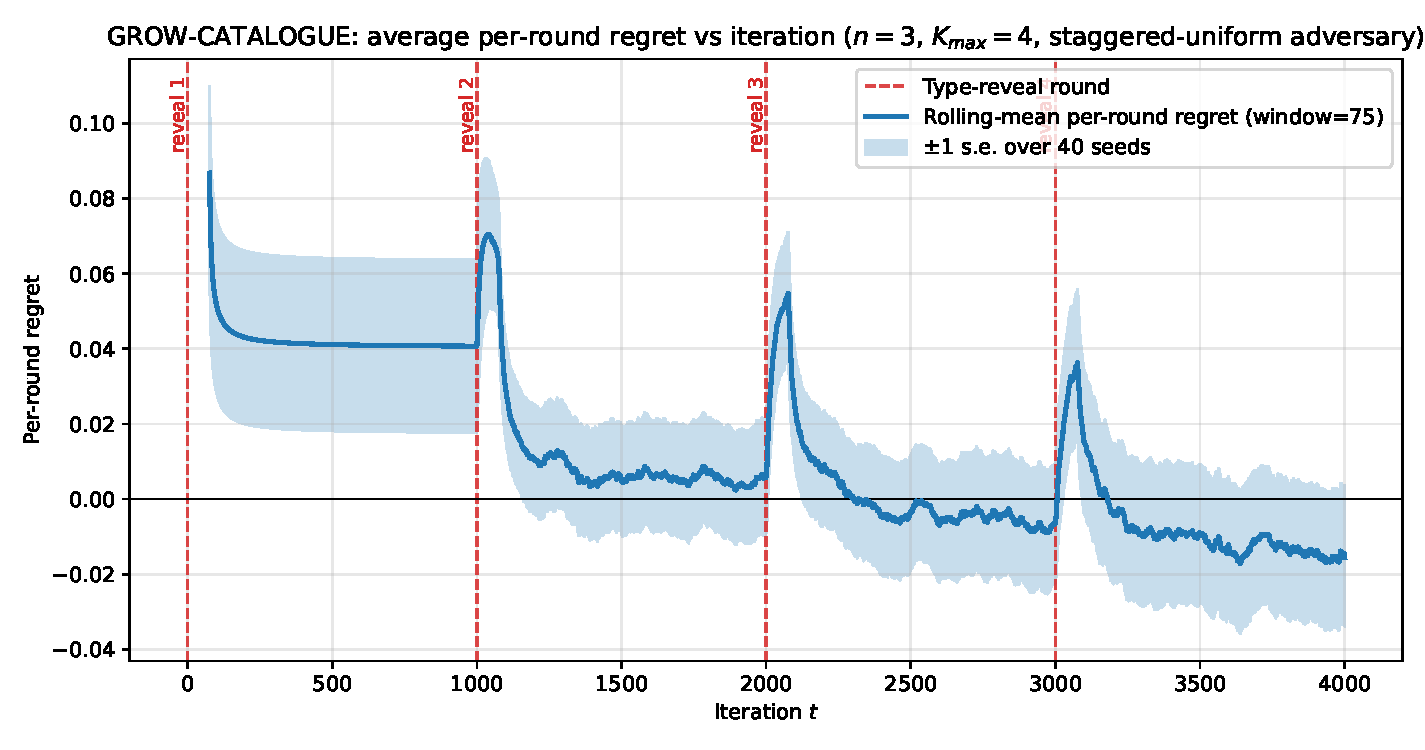
\includegraphics[width=0.98\linewidth]{figures/avg_regret_per_iter.pdf}
\vspace{-0.5em}
\caption{Rolling-window per-round regret of \textsc{Grow-Catalogue} under
the staggered-uniform adversary ($n=3$, $\Kmax=4$, $T=4000$, average over
$40$ seeds, window $=75$). Red dashed lines mark the discovery rounds
$0,1000,2000,3000$. Each reveal causes a visible transient spike,
followed by PW re-convergence inside the new epoch.}
\label{fig:per-round}
\end{figure}

\begin{figure}[t]
\centering
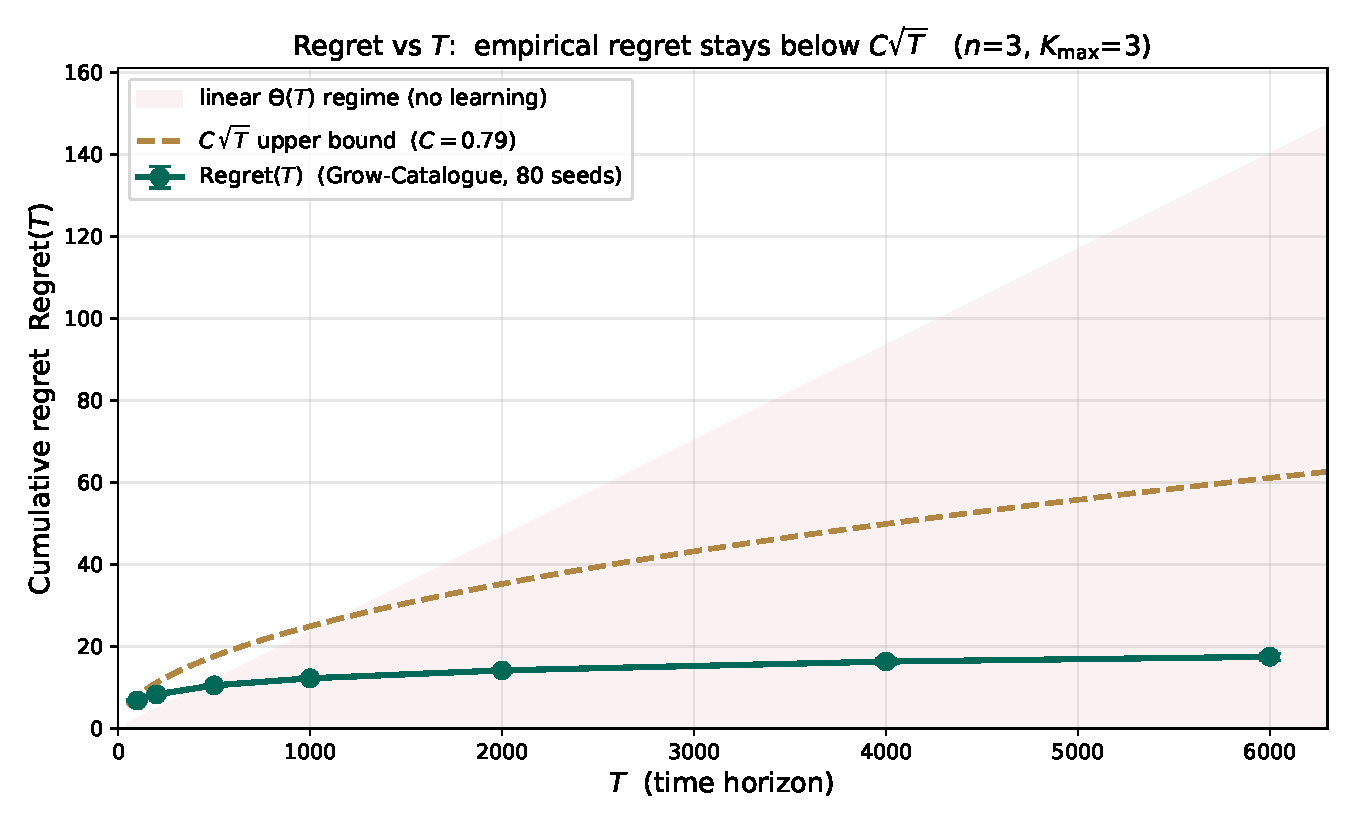
\includegraphics[width=0.98\linewidth]{figures/regret_vs_T_scaling.pdf}
\vspace{-0.5em}
\caption{Cumulative regret versus horizon $T$ for \textsc{Grow-Catalogue}
($n=3$, $\Kmax=3$, uniform random adversary, 80 seeds). The green curve
stays strictly below the $C\sqrt T$ upper envelope implied by
\Cref{thm:main}, which is in turn well below the linear-regret regime
that would result without learning.}
\label{fig:scaling}
\end{figure}

\Cref{fig:per-round} shows that the algorithm's per-round regret tracks
the epoch structure of the proof: each discovery round produces a bounded
transient, and the PW sub-routine re-converges within the new epoch. The
spikes shrink with $i$ because, by epoch $i$, the algorithm already has a
good PW distribution on most of the new (refined) extreme points.

\Cref{fig:scaling} plots cumulative $\Regret(T)$ versus $T$ with the
$C\sqrt T$ envelope from \Cref{thm:main} overlaid. The empirical regret
stays visibly below the envelope for all $T$ tested, and the ratio
$\Regret(T)/\sqrt T$ remains bounded (in fact, it decreases, indicating
that the stochastic staggered-uniform adversary is far from the worst
case). This is entirely consistent with \Cref{thm:main}, which is our upper bound

\Cref{tab:comparison} compares the four algorithms at $T=4000$. The regret
of \textsc{Grow-Catalogue} is
within roughly $15\%$--$40\%$ of the known-$K$ oracle and an order of
magnitude better than the uniform baseline. The two \textsc{Grow-Catalogue}
variants produce regret that differs only by Monte-Carlo noise, as
predicted by the observational equivalence of the two recomputation
schemes.

\begin{table}[h]
\centering
\footnotesize
\renewcommand{\arraystretch}{1.15}
\begin{tabular}{lcc}
\toprule
Algorithm & $\EE[\Regret(T)]$ & Ratio\\
\midrule
Known-$K$ oracle of \citet{balcan2015} & $14.51\pm 5.00$  & $1.00$\\
\textsc{Grow-Cat.} (total)     & $16.57\pm 5.40$  & $1.14$\\
Uniform baseline               & $292.77\pm 350.28$ & $20.18$\\
\bottomrule
\end{tabular}
\caption{Cumulative regret at $T=4000$, $n=3$, $\Kmax=3$, uniform-random
adversary, mean $\pm$ std over 15 seeds. The known-$K$ oracle receives
$K$ in advance; \textsc{Grow-Catalogue} attains comparable regret
\emph{without} this information.}
\label{tab:comparison}
\end{table}

% ==========================================================================
\section{Conclusions}
\label{sec:conc}

We studied the repeated Stackelberg security game in a new, open regime
in which the set of attacker types is unknown to the defender a priori
but known to have bounded cardinality. We presented \textsc{Grow-Catalogue},
a simple online algorithm that incrementally discovers attacker types and
re-partitions the coverage polytope accordingly, and we gave a full proof
that its expected regret under full-information feedback is at most
$O\!\bigl(\sqrt{T\cdot\Kmax\cdot(n^2+\Kmax\log n)}\bigr)$. This is the
same functional form as the known-$K$ bound of \citet[Theorem 5.1]{balcan2015},
with the known cardinality $k$ replaced by our known upper bound $\Kmax$.
The bound is sublinear whenever $\Kmax\cdot(n^2+\Kmax\log n)=o(T)$, and
the matching $\Omega(T)$ lower bound of \citet[Theorem 7.1]{balcan2015}
rules out further improvements on the unbounded side. Our experiments
confirm the analytical scaling: the empirical regret stays below the
$C\sqrt T$ envelope and tracks the epoch structure of the proof.



\bibliography{refs}




\end{document}
